\documentclass{beamer}
\usepackage[english]{babel}
\usepackage[utf8]{inputenc}
\usepackage[T1]{fontenc}

\usepackage{amsmath} % math stuff
\usepackage{amssymb} % math stuff
\usepackage{amsthm}  % math stuff
\usepackage{commath} % math stuff
\usepackage{relsize} % math stuff
\usepackage{caption} % caption stuff
\usepackage{graphicx} % images
\usepackage{listings} % code listings
\usepackage{courier} % courier font
\usepackage{enumerate}
\usepackage{mathtools}
\usepackage{float}
\usepackage{cite}

%tikz
\usepackage{tikz}
\usetikzlibrary{arrows,automata,positioning}

\title{Getting robots bored enough to move cubes}
\author{Julien Scholz}
\date{June 16, 2020}

\begin{document}

\frame{\titlepage}

\begin{frame}{Ingredients for bored robots}
    \begin{itemize}
        \item Reinforcement learning with intrinsic rewards
        \item Model of the environment
        \item Continuous actions
        \item A planning algorithm to deal with sensorimotor delays and prevent irreversable actions
    \end{itemize}
\end{frame}

\begin{frame}{MuZero Algorithm \cite{muzero}}
    \begin{figure}
        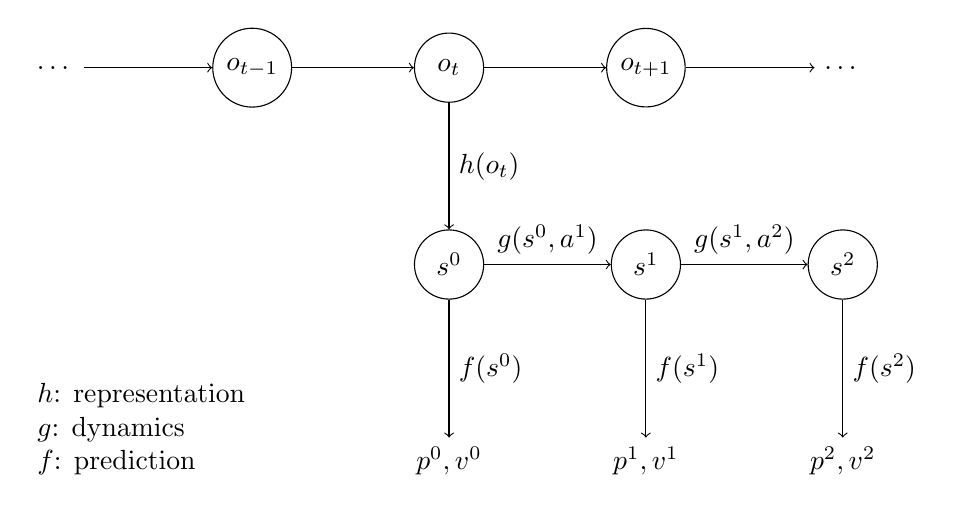
\begin{tikzpicture}[->,auto,node distance=2.5cm]
            \node (ellipsis_left) {\dots};
            \node[state] (o_t-1) [right of=ellipsis_left] {$o_{t-1}$};
            \node[state] (o_t) [right of=o_t-1] {$o_t$};
            \node[state] (o_t1) [right of=o_t] {$o_{t+1}$};
            \node (ellipsis_right) [right of=o_t1] {\dots};

            \path (ellipsis_left) edge node {} (o_t-1);
            \path (o_t-1) edge node {} (o_t);
            \path (o_t) edge node {} (o_t1);
            \path (o_t1) edge node {} (ellipsis_right);

            \node[state] (s_0) [below of=o_t] {$s^0$};
            \node[state] (s_1) [right of=s_0] {$s^1$};
            \node[state] (s_2) [right of=s_1] {$s^2$};

            \path (o_t) edge node {$h(o_t)$} (s_0);

            \path (s_0) edge node {$g(s^0, a^1)$} (s_1);
            \path (s_1) edge node {$g(s^1, a^2)$} (s_2);

            \node (v_0) [below of=s_0] {$p^0, v^0$};
            \node (v_1) [below of=s_1] {$p^1, v^1$};
            \node (v_2) [below of=s_2] {$p^2, v^2$};

            \path (s_0) edge node {$f(s^0)$} (v_0);
            \path (s_1) edge node {$f(s^1)$} (v_1);
            \path (s_2) edge node {$f(s^2)$} (v_2);

            \node[align=left] (desc) at (current bounding box.south west) [anchor=south west] {$h$: representation \\ $g$: dynamics \\ $f$: prediction};
        \end{tikzpicture}
    \end{figure}
\end{frame}


\begin{frame}{References}
\bibliography{bibliography}
\bibliographystyle{plain}
\end{frame}

\end{document}